\problemname{Dandelions}
\noindent
During his youth, Gösta was quite fond of dandelion soda. 
Unfortunately, it's not popular at all anymore. 
In his older age, Gösta has become wealthy, and he now wants to use his fortune to open a business selling dandelion soda. 
To do this, he will obviously need a lot of dandelions. He has a meadow that is $R \times C$ square meters in size. 
It is well known that dandelions do not thrive if they grow close to each other. 
More precisely, if the meadow is divided into squares of size $1 \times 1$ meter, at most one dandelion can grow within each.

Currently, there are dandelions growing in $N$ cells. 
Gösta wants his meadow to have a dandelion in every square. 
Once a year, the dandelions bloom, and he can then use a large fan to blow from either the west, east, north, or south. 
Each blooming dandelion's seeds will then move one square in the direction of the wind. 
If the square it lands on is empty, a dandelion will grow there next year. 
If there is already a dandelion on a square, it will remain there next year as well. 
Since Gösta doesn't have many years left, he wants to calculate the number of years it will take to fill the entire meadow with dandelions if he chooses the optimal wind directions.


\section*{Input}
\noindent
The first line contains the integers $R$ and $C$ ($1 \leq R,C \leq 10^9$), the number of rows and columns in the grid.

Following that is a line with the integer $N$ ($1 \leq N \leq 300$), the number of dandelions currently in the meadow.

The next $N$ lines contain the integers $r_i$ and $c_i$ ($1 \leq r_i \leq R$, $1 \leq c_i \leq C$), 
indicating that initially there is a dandelion in the cell ($r_i, c_i$). Initially, two dandelions never grow on the same square.

\section*{Output}
\noindent
Print an integer: the minimum number of years to fill the entire meadow with dandelions if the wind directions are chosen optimally.

\section*{Scoring}
Your solution will be tested on a set of test groups, each worth a number of points. 
Each test group contains a set of test cases. 
To get the points for a test group you need to solve all test cases in the test group.

\noindent
\begin{tabular}{| l | l | p{12cm} |}
  \hline
  \textbf{Group} & \textbf{Point value} & \textbf{Constraints} \\ \hline
  $1$    & $5$          & $R,C \leq 4$  \\ \hline
  $2$    & $10$         & $R,C \leq 40$ \\ \hline
  $3$    & $15$         & $R \leq 40$ \\ \hline
  $4$    & $30$         & $N \leq 25$ \\ \hline
  $5$    & $20$         & $N \leq 100$ \\ \hline
  $6$    & $20$         & No additional constraints. \\ \hline
\end{tabular}



\section*{Explanation of sample 1:}
Initially, there are dandelions on the following squares:
\begin{centering}
  \begin{figure}[h]
      \centering
      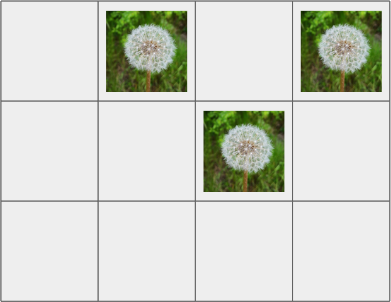
\includegraphics[width=0.8\textwidth]{t0.png}
  \end{figure}
\end{centering}
If we blow the wind from the south, the dandelions spread to the west:
\begin{centering}
  \begin{figure}[h]
      \centering
      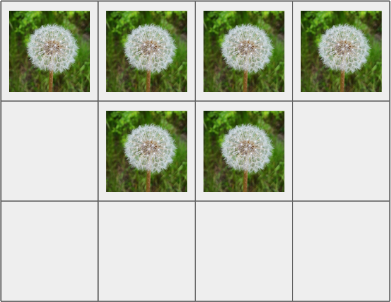
\includegraphics[width=0.8\textwidth]{t1.png}
  \end{figure}
\end{centering}
If we then blow the wind from the north, the dandelions spread southward:
\begin{centering}
  \begin{figure}[h]
      \centering
      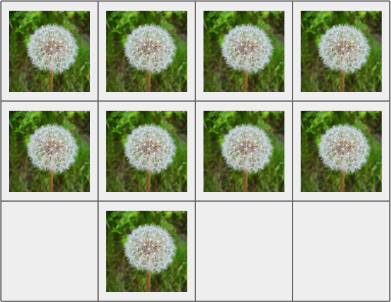
\includegraphics[width=0.8\textwidth]{t2.png}
  \end{figure}
\end{centering}
If we blow the wind from the north once again, the entire meadow will be filled.
\begin{centering}
  \begin{figure}[h]
      \centering
      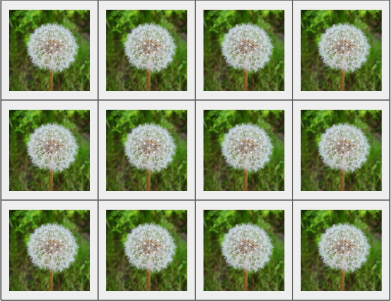
\includegraphics[width=0.8\textwidth]{t3.png}
  \end{figure}
\end{centering}
